\documentclass[conference]{IEEEtran}
\IEEEoverridecommandlockouts
% The preceding line is only needed to identify funding in the first footnote. If that is unneeded, please comment it out.
%Template version as of 6/27/2024

\usepackage{cite}
\usepackage{amsmath,amssymb,amsfonts}
\usepackage{algorithmic}
\usepackage{algorithm,float}
\usepackage{array}
\usepackage{graphicx}
\usepackage{textcomp}
\usepackage{xcolor}
\usepackage{stfloats}
\usepackage{url}
\usepackage{verbatim}
\usepackage{subfig}
\usepackage{cite}
\usepackage{booktabs}
\usepackage{tabularx}
\usepackage{gensymb}
\usepackage{listings}

\def\BibTeX{{\rm B\kern-.05em{\sc i\kern-.025em b}\kern-.08em
    T\kern-.1667em\lower.7ex\hbox{E}\kern-.125emX}}
\begin{document}

\title{Q-band ART: Adaptive Band Suppression for Anti-Rollover Tracking of Semi-Trailer Tank Trucks
\thanks{This work was supported by the National Key R\&D Program of China (2021YFB2501000).\textit{(Corresponding author: Wei Zhong.)}}
}

\author{\IEEEauthorblockN{1\textsuperscript{st} Xiaojing Qi}
\IEEEauthorblockA{\textit{School of Vehicle and Mobility} \\
\textit{Tsinghua University}\\
Beijing, China \\
komasaqi@foxmail.com}
\and
\IEEEauthorblockN{2\textsuperscript{nd} Linhao Gong}
\IEEEauthorblockA{\textit{School of Automotive and Traffic Engineering} \\
\textit{Jiangsu University of Technology}\\
Changzhou, China \\
linhaogong6@gmail.com}
\and
\IEEEauthorblockN{3\textsuperscript{rd} Kunpeng Wang}
\IEEEauthorblockA{\textit{School of Automotive Studies} \\
\textit{Chang'an University}\\
Xian, China \\
15389694186@163.com}
\and
\IEEEauthorblockN{4\textsuperscript{th} Wei Zhong}
\IEEEauthorblockA{\textit{State Key Laboratory of Intelligent Green} \\
\textit{Vehicle and Mobility,Tsinghua University}\\
Beijing, China \\
zhongwei@mail.tsinghua.edu.cn}
\and
\IEEEauthorblockN{5\textsuperscript{th} Bolin Gao}
\IEEEauthorblockA{\textit{School of Vehicle and Mobility} \\
\textit{Tsinghua University}\\
Beijing, China \\
gaobolin@tsinghua.edu.cn}
\and
\IEEEauthorblockN{6\textsuperscript{th} Yugong Luo}
\IEEEauthorblockA{\textit{School of Vehicle and Mobility} \\
\textit{Tsinghua University}\\
Beijing, China \\
lyg@tsinghua.edu.cn}
}

\maketitle

\providecommand{\Qband}{\ensuremath{Q_{\mathrm{band}}}}
\providecommand{\ay}{\ensuremath{a_y}}
\providecommand{\LTR}{\ensuremath{\mathrm{LTR}}}
\providecommand{\T}{\ensuremath{\mathrm{T}}}

\begin{abstract}
Semi-trailer tankers are prone to rollover because lateral acceleration excites both suspension roll and liquid sloshing. Existing anti-rollover tracking methods usually introduce liquid states, roll states, or lateral load transfer ratio predictions into model predictive control, which increases dependence on liquid calibration, trailer-side sensing, and online model dimension. This paper proposes Q-band ART, an adaptive band-suppression framework that penalizes the predicted lateral-acceleration energy in rollover-critical frequency bands. A reduced cart-roll-sloshing model explains why the critical band should be identified from the coupled acceleration-to-risk response, rather than from an isolated liquid or roll natural frequency. The resulting Q-band term is embedded into a tracking controller with acceleration smoothing, soft band constraints, preview-adaptive weights, extended-state disturbance compensation, and hitch-angle-based parameter scheduling. The method is validated in 5-pins simulations and 1:14 model-truck experiments, reducing peak rollover-risk proxy from xxx to xxx while maintaining acceptable tracking error and real-time performance.
\end{abstract}

\begin{IEEEkeywords}
Anti-rollover control, semi-trailer tanker, liquid sloshing, path tracking, model predictive control, frequency-band suppression.
\end{IEEEkeywords}


\section{Introduction}
\IEEEPARstart{S}{emi-trailer} tank trucks are indispensible for liquid hazardous-chemical logistics, but their  partially filled tanks make rollover a severe safety risk. Accident reports show that tank truck rollovers are often triggered by sharp steering, emergency avoidance, curved-road overspeed, or driver error, and may lead to deadly secondary disasters \cite{chengshuo2023,wangyang2023,wenling_accident2022}. Because safety standards leave practical operation across partial filling rates \cite{biaozhun185642006,biaozhunR00052011}, free-surface sloshing must be considered in autonomous tank truck tracking.

Studies show that with free-surface, driving excitations generate additional sloshing, making medium filling rates yielding stronger dynamic instability than either empty or fully filled cases. And the sloshing in tank has been modeled by quasi-static centroid-shift methods, mechanical equivalent models (MEMs), computational fluid dynamics, and experiments. \cite{maohaijian2021fsi,huangyang2017impact,wanying2020antirolover,wangxiaorun2022lateralacc,chenyibao2016crosssection}. Among the methods, MEMs especially pendulum models are widely used for their ability to balance interpretability and real-time computation, although the dominant sloshing modes still require accurate calibration \cite{jiaxinhong2022review,salem2000rollover,yangxiujian2018multimass,Komasa2023observing}.

For semi-trailer tank trucks, rollover prevention is further complicated by tractor-trailer articulation. High-fidelity models may include lateral, yaw, and roll motion of tractor and trailer,respectively, as well as liquid states \cite{renyuanyuan2020precisemodel,yuzhixin2018mpc,zongchangfu2014identification,niezhigen2015heavyduty}. Such models are useful offline, but online use is limited by trailer replacement, non-unified trailer interfaces, limited trailer-side sensing, and uncertain liquid/suspension parameters. Active suspension, steering, and differential braking have all been studied for rollover prevention \cite{xiao2020rollsuspension,carlson2003rollover,xu2011rollover}; tank truck-specific controllers have used PID, LQR, MPC, model-free adaptive control (MFAC), and other robust control with MEMs \cite{zhaoweiqiang2018equivalent,zhaoweiqiang2019semitrailer,Reviewer2_SunWencai2022,MFAC_LiXiansheng2021,zhao2019hinfty,KomasaQi2025AntiRollover_TITS}.

Most existing controllers still rely on explicit liquid states, roll states, or lateral load transfer ratio (LTR) predictions. This is not always suitable for autonomous semi-trailer tank trucks with limited trailer sensing and embedded computing resources. Model predictive control (MPC) can combine tracking, actuator, acceleration, and safety constraints \cite{gongjianwei2020mpcbook}, but high-dimensional states and dense constraints challenge real-time implementation \cite{shengbo2015fastmpc}. This paper therefore suppresses rollover excitation from the input side: the predicted lateral-acceleration sequence is projected onto vehicle-liquid critical bands, and the resulting energy is penalized and softly constrained. The workflow is shown in Fig.~\ref{fig:intro_architecture}.

\begin{figure*}[!t]
\centering
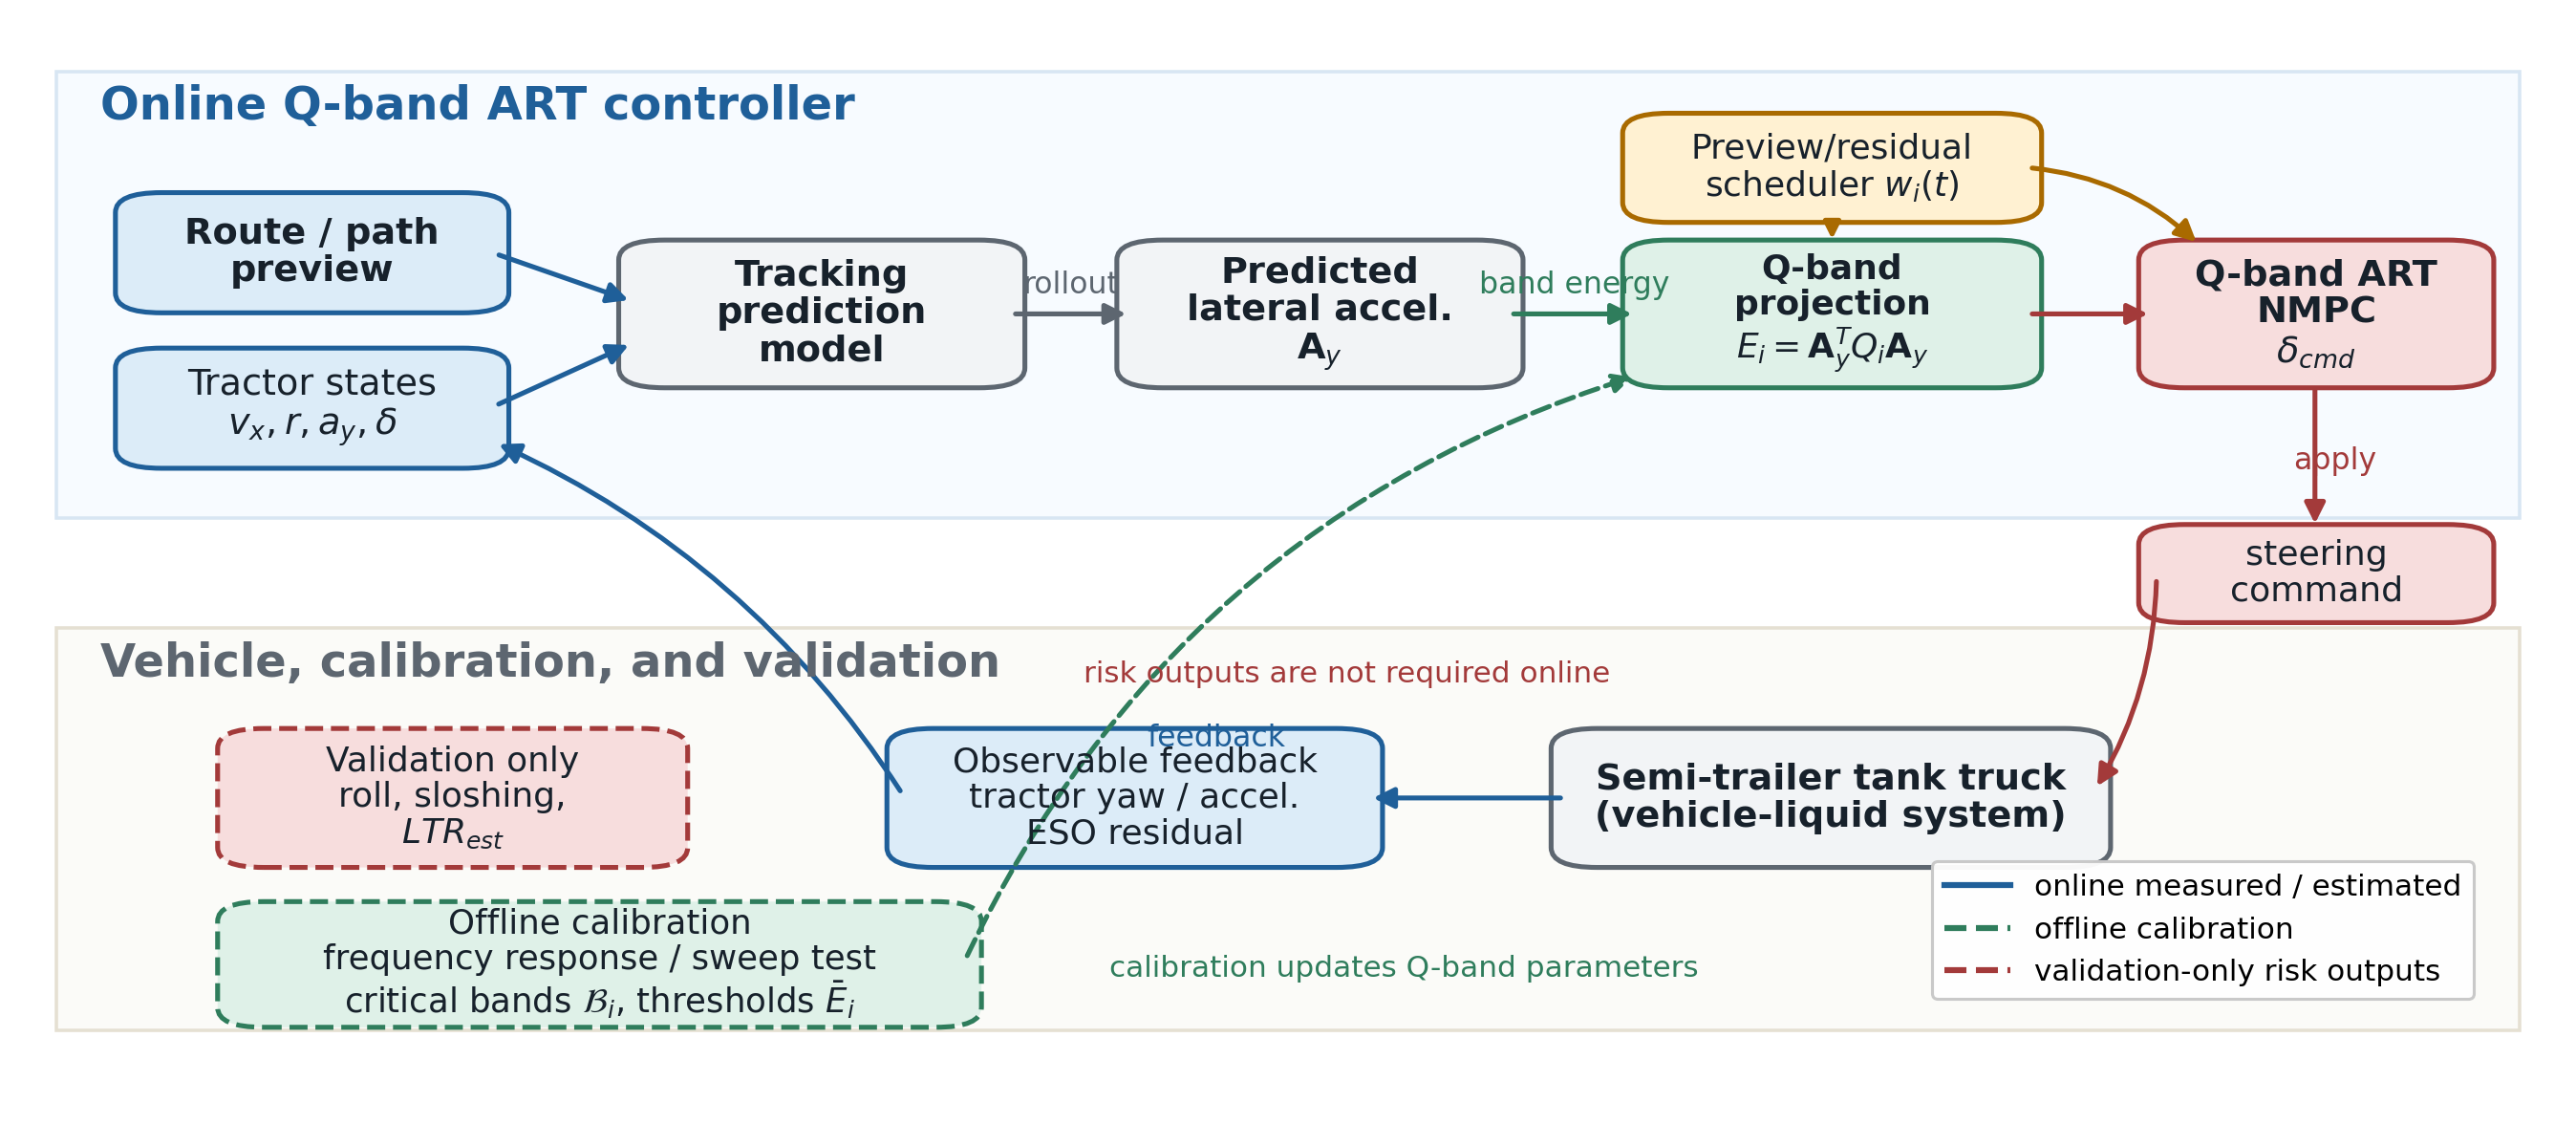
\includegraphics[width=0.98\textwidth]{fig/intro_architecture.png}
\caption{Architecture of Q-band ART. Offline calibration identifies the critical bands, energy thresholds, Q-band matrices, and conservative margins. The online controller then combines tractor-side prediction, ESO residual compensation, hitch-angle-based equivalent-parameter scheduling, Q-band projection, and NMPC to output steering commands using tractor-side sensing and precomputed Q-band parameters.}
\label{fig:intro_architecture}
\end{figure*}


The contributions are threefold. First, a Q-band anti-excitation view is introduced for semi-trailer tank truck tracking, avoiding mandatory online liquid-state modeling and observation. Second, an multi-point NMPC tracking controller with disturbance compensation and trailer-free modeling is designed specifically for semi-trailer. Third, the Q-band term is integrated predictively into the controller for anti-rollover purpose and validated through simulation and 1:14 model-truck experiments. The rest of the paper presents the model, controller, validation, and conclusions. 


\section{Q-Band-Oriented Modeling}

\subsection{Reduced Roll-Sloshing Excitation Model}
Q-band ART does not require the online controller to predict the full liquid state. A reduced model is used only to explain which lateral-acceleration components are dangerous. The unsprung/base motion is represented by a lateral cart, the sprung tank body by a roll pendulum, and the dominant liquid mode by a pendulum attached to the tank body. Let
\begin{equation}
    \mathbf{x}_r=[\phi,\theta]^\T ,
\end{equation}
where $\phi$ is the tank-body roll angle and $\theta$ is the relative liquid sloshing angle. Around a nominal operating point, the coupled roll-sloshing dynamics can be written as
\begin{equation}
    \mathbf{M}\ddot{\mathbf{x}}_r+\mathbf{C}\dot{\mathbf{x}}_r+\mathbf{K}\mathbf{x}_r=\mathbf{B}_a \ay ,
    \label{eq:reduced_roll_slosh}
\end{equation}
where $\ay$ is the lateral acceleration generated by steering and tracking. The off-diagonal terms in $\mathbf{M}$ and $\mathbf{K}$ describe the coupling between suspension roll and liquid motion. Therefore, the dangerous frequency is not necessarily the isolated liquid natural frequency or the isolated roll frequency.

\begin{figure}[!t]
\centering
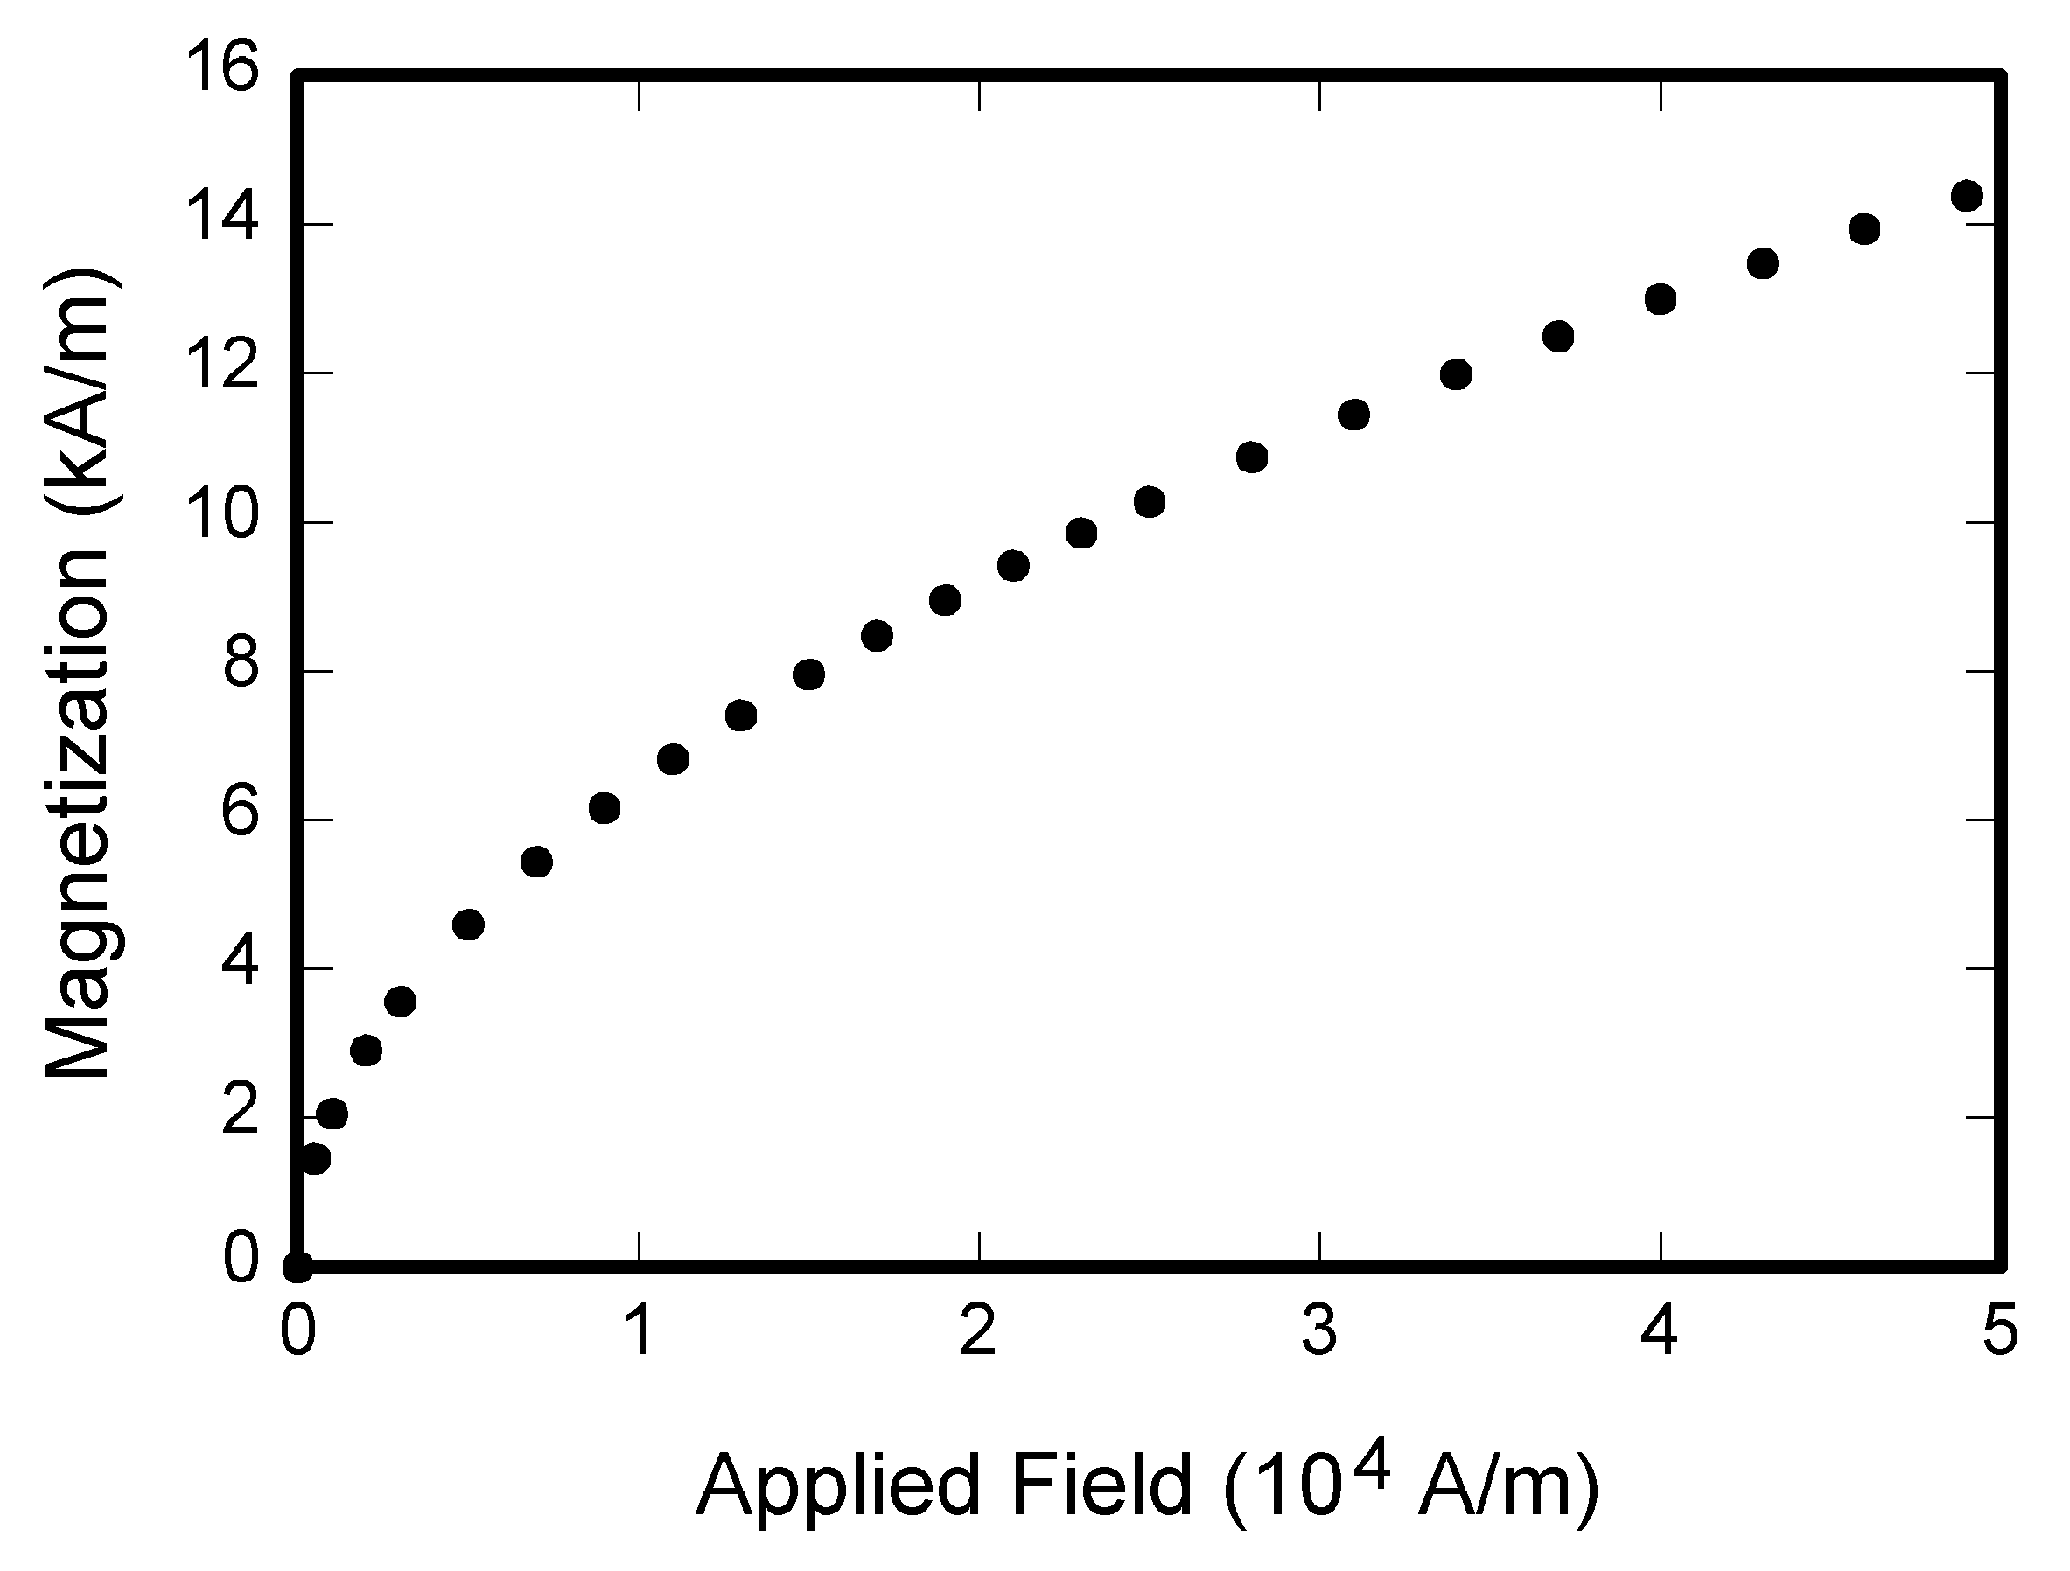
\includegraphics[width=\linewidth]{fig/fig1.png}
\caption{Reduced lateral model used to derive the Q-band concept. The online controller only needs the predicted lateral acceleration, while roll, sloshing, and LTR-related quantities are used for interpretation and validation.}
\label{fig:simplified_model}
\end{figure}
% TODO（作者）：将 fig1.png 替换为简化侧向模型图。建议左侧画半挂液罐车，右侧画小车-悬架倒立摆-液体正摆；标注 a_y、phi、theta、risk output。不要放太多参数，避免会议论文图太拥挤。

\subsection{Critical Band and Risk Bound}
Let the rollover-risk output be
\begin{equation}
    z=C_z\mathbf{x}_r+D_z\ay ,
\end{equation}
where $z$ can represent dynamic LTR, roll moment, roll-rate-weighted risk, or another calibrated rollover proxy. From \eqref{eq:reduced_roll_slosh}, the input-output frequency response is
\begin{equation}
    G_{za}(s)=C_z(s^2\mathbf{M}+s\mathbf{C}+\mathbf{K})^{-1}\mathbf{B}_a+D_z .
    \label{eq:freq_response}
\end{equation}
The Q-band $\mathcal{B}_i=[f_i^-,f_i^+]$ is selected around the peak or broad-peak region of $|G_{za}(j2\pi f)|$. In this work the main band is centered on the dominant sloshing-related response, with additional bands covering secondary and higher-frequency coupled excitations.

The following frequency-domain argument explains the safety meaning of Q-band suppression. If $|G_{za}(j2\pi f)|\leq \bar{G}_{\mathcal{B}}$ in a target band and the input component in that band has energy $\|a_{y,\mathcal{B}}\|_2^2$, then
\begin{equation}
    \|z_{\mathcal{B}}\|_2 \leq \bar{G}_{\mathcal{B}}\|a_{y,\mathcal{B}}\|_2 .
\end{equation}
Thus, limiting the band energy of $\ay$ gives a conservative bound on the risk output caused by that band. This is a sufficient safety explanation, not a replacement for full vehicle validation.

% TODO（作者）：最终稿需要给出由扫频、TruckSim 或模型车辨识得到的危险频带。当前 MATLAB 脚本采用 0.35--0.75 Hz 作为主频带，并覆盖 0.75--1.45 Hz 等次级频段；后续应写清楚这些频段的标定来源。

\subsection{Tracking Model and Disturbance Compensation}
For online tracking, the controller uses a low-dimensional prediction model that provides $\mathbf{A}_y$ over the horizon. In the engineering implementation, this prediction layer can be a kinematic or two-degree-of-freedom tractor model, while the validation object is the semi-trailer tank truck model in TruckSim and the model-truck platform. For the dynamic version,
\begin{equation}
\begin{aligned}
    \dot v_y &= \frac{F_{yf}\cos\delta+F_{yr}}{m_{\mathrm{eq}}}-v_xr+d_y,\\
    \dot r &= \frac{l_fF_{yf}\cos\delta-l_rF_{yr}}{I_{z,\mathrm{eq}}}+d_r,
\end{aligned}
\label{eq:tractor_2dof}
\end{equation}
where $d_y$ and $d_r$ collect trailer force, liquid sloshing, tire mismatch, and parameter error. An extended-state observer estimates the dominant residual, and a hitch-angle estimator schedules $m_{\mathrm{eq}}$ and $I_{z,\mathrm{eq}}$ as low-frequency articulated-vehicle priors. The remaining unmodeled dynamics are handled by safety margins and Q-band suppression rather than by adding liquid states to the optimizer.

\subsection{Online and Offline Quantities}
The online Q-band controller depends on predicted lateral acceleration, vehicle speed, steering state, yaw response, and reference preview. Liquid angle, true wheel loads, and high-fidelity LTR are not required online. They are used offline to calibrate the dangerous bands and to evaluate simulation or model-truck safety. This separation is important for trailer-sensing-limited deployment.


\section{Adaptive Q-Band Suppression Controller}

\subsection{Band-Energy Projection}
Let the prediction horizon contain $N$ samples and sampling time $\Delta t$. The predicted lateral-acceleration sequence is
\begin{equation}
    \mathbf{A}_y=[a_{y,0},a_{y,1},\ldots,a_{y,N-1}]^\T .
\end{equation}
For a critical band $\mathcal{B}_i$, choose discrete frequencies $f_{ij}$ and time grid $t_k=k\Delta t$. Define
\begin{equation}
    \mathbf{c}_{ij}=[\cos(2\pi f_{ij}t_0),\ldots,\cos(2\pi f_{ij}t_{N-1})]^\T ,
\end{equation}
\begin{equation}
    \mathbf{s}_{ij}=[\sin(2\pi f_{ij}t_0),\ldots,\sin(2\pi f_{ij}t_{N-1})]^\T .
\end{equation}
The band energy is
\begin{equation}
    E_i(\mathbf{A}_y)=\mathbf{A}_y^\T\mathbf{Q}_i\mathbf{A}_y,
\end{equation}
\begin{equation}
    \mathbf{Q}_i=\frac{1}{N^2}\sum_j(\mathbf{c}_{ij}\mathbf{c}_{ij}^\T+\mathbf{s}_{ij}\mathbf{s}_{ij}^\T)\succeq0 .
\end{equation}
The matrix $\mathbf{Q}_i$ can be precomputed for fixed $\Delta t$, $N$, and $\mathcal{B}_i$. Hence the Q-band term adds no new vehicle state; it only reshapes the predicted lateral acceleration.

\subsection{Optimization Problem}
The Q-band ART objective combines tracking, actuator regularization, acceleration smoothing, and band suppression:
\begin{equation}
\begin{aligned}
\min_{\mathbf{U},\mathbf{S}}~&
J_{\mathrm{trk}}+J_u+J_{\Delta u}
w_a\|\mathbf{A}_y\|_2^2+w_1\|\mathbf{D}_1\mathbf{A}_y\|_2^2\\
&+w_2\|\mathbf{D}_2\mathbf{A}_y\|_2^2
\sum_i w_i(t)\mathbf{A}_y^\T\mathbf{Q}_i\mathbf{A}_y
\sum_i\rho_i s_i^2 ,
\end{aligned}
\label{eq:qband_cost}
\end{equation}
where $\mathbf{D}_1$ and $\mathbf{D}_2$ are first- and second-order difference matrices. The constraints are
\begin{equation}
\begin{aligned}
    \mathbf{x}_{k+1}&=f(\mathbf{x}_k,u_k,\hat d_k),\\
    |a_{y,k}|&\leq a_{y,\max}^{\mathrm{dyn}},\\
    u_{\min}&\leq u_k\leq u_{\max},\quad |\Delta u_k|\leq \Delta u_{\max},\\
    E_i(\mathbf{A}_y)&\leq \bar{E}_i+s_i,\quad s_i\geq0 .
\end{aligned}
\label{eq:qband_constraints}
\end{equation}
The soft band constraint prevents the optimizer from concentrating energy in a dangerous band, while preserving feasibility when the reference path is aggressive. In low-risk segments, $w_i(t)$ remains small and the controller behaves like a normal tracker.

\subsection{Preview-Adaptive Scheduling}
Pure feedback scheduling raises the safety weight only after the roll-slosh response has already been excited. Q-band ART uses preview risk as the main trigger. A reference lateral-acceleration sequence $\mathbf{A}_{y,\mathrm{ref}}$ is computed from the future path or curvature, and its band energy is compared with the calibrated threshold:
\begin{equation}
    R_i^{\mathrm{pre}}=\max\left(0,\frac{\mathbf{A}_{y,\mathrm{ref}}^\T\mathbf{Q}_i\mathbf{A}_{y,\mathrm{ref}}}{\bar{E}_{i,\mathrm{ref}}}-1\right).
\end{equation}
The raw weight is scheduled as
\begin{equation}
    w_i^{\mathrm{raw}}=w_i^{\min}+
    \left(1-e^{-\kappa R_i^{\mathrm{pre}}}\right)(w_i^{\mathrm{tar}}-w_i^{\min}).
\end{equation}
Observed yaw or roll residuals can further increase the weight when residual sloshing remains. A non-symmetric filter is then applied:
\begin{equation}
    w_i(t)=(1-\alpha_i)w_i(t-\Delta t)+\alpha_i w_i^{\mathrm{raw}},
\end{equation}
where $\alpha_i=\alpha_\uparrow$ if $w_i^{\mathrm{raw}}>w_i(t-\Delta t)$ and $\alpha_i=\alpha_\downarrow$ otherwise. With $\alpha_\uparrow>\alpha_\downarrow$, the weight rises before a high-risk lane change and decays slowly after it.

\begin{figure}[!t]
\centering
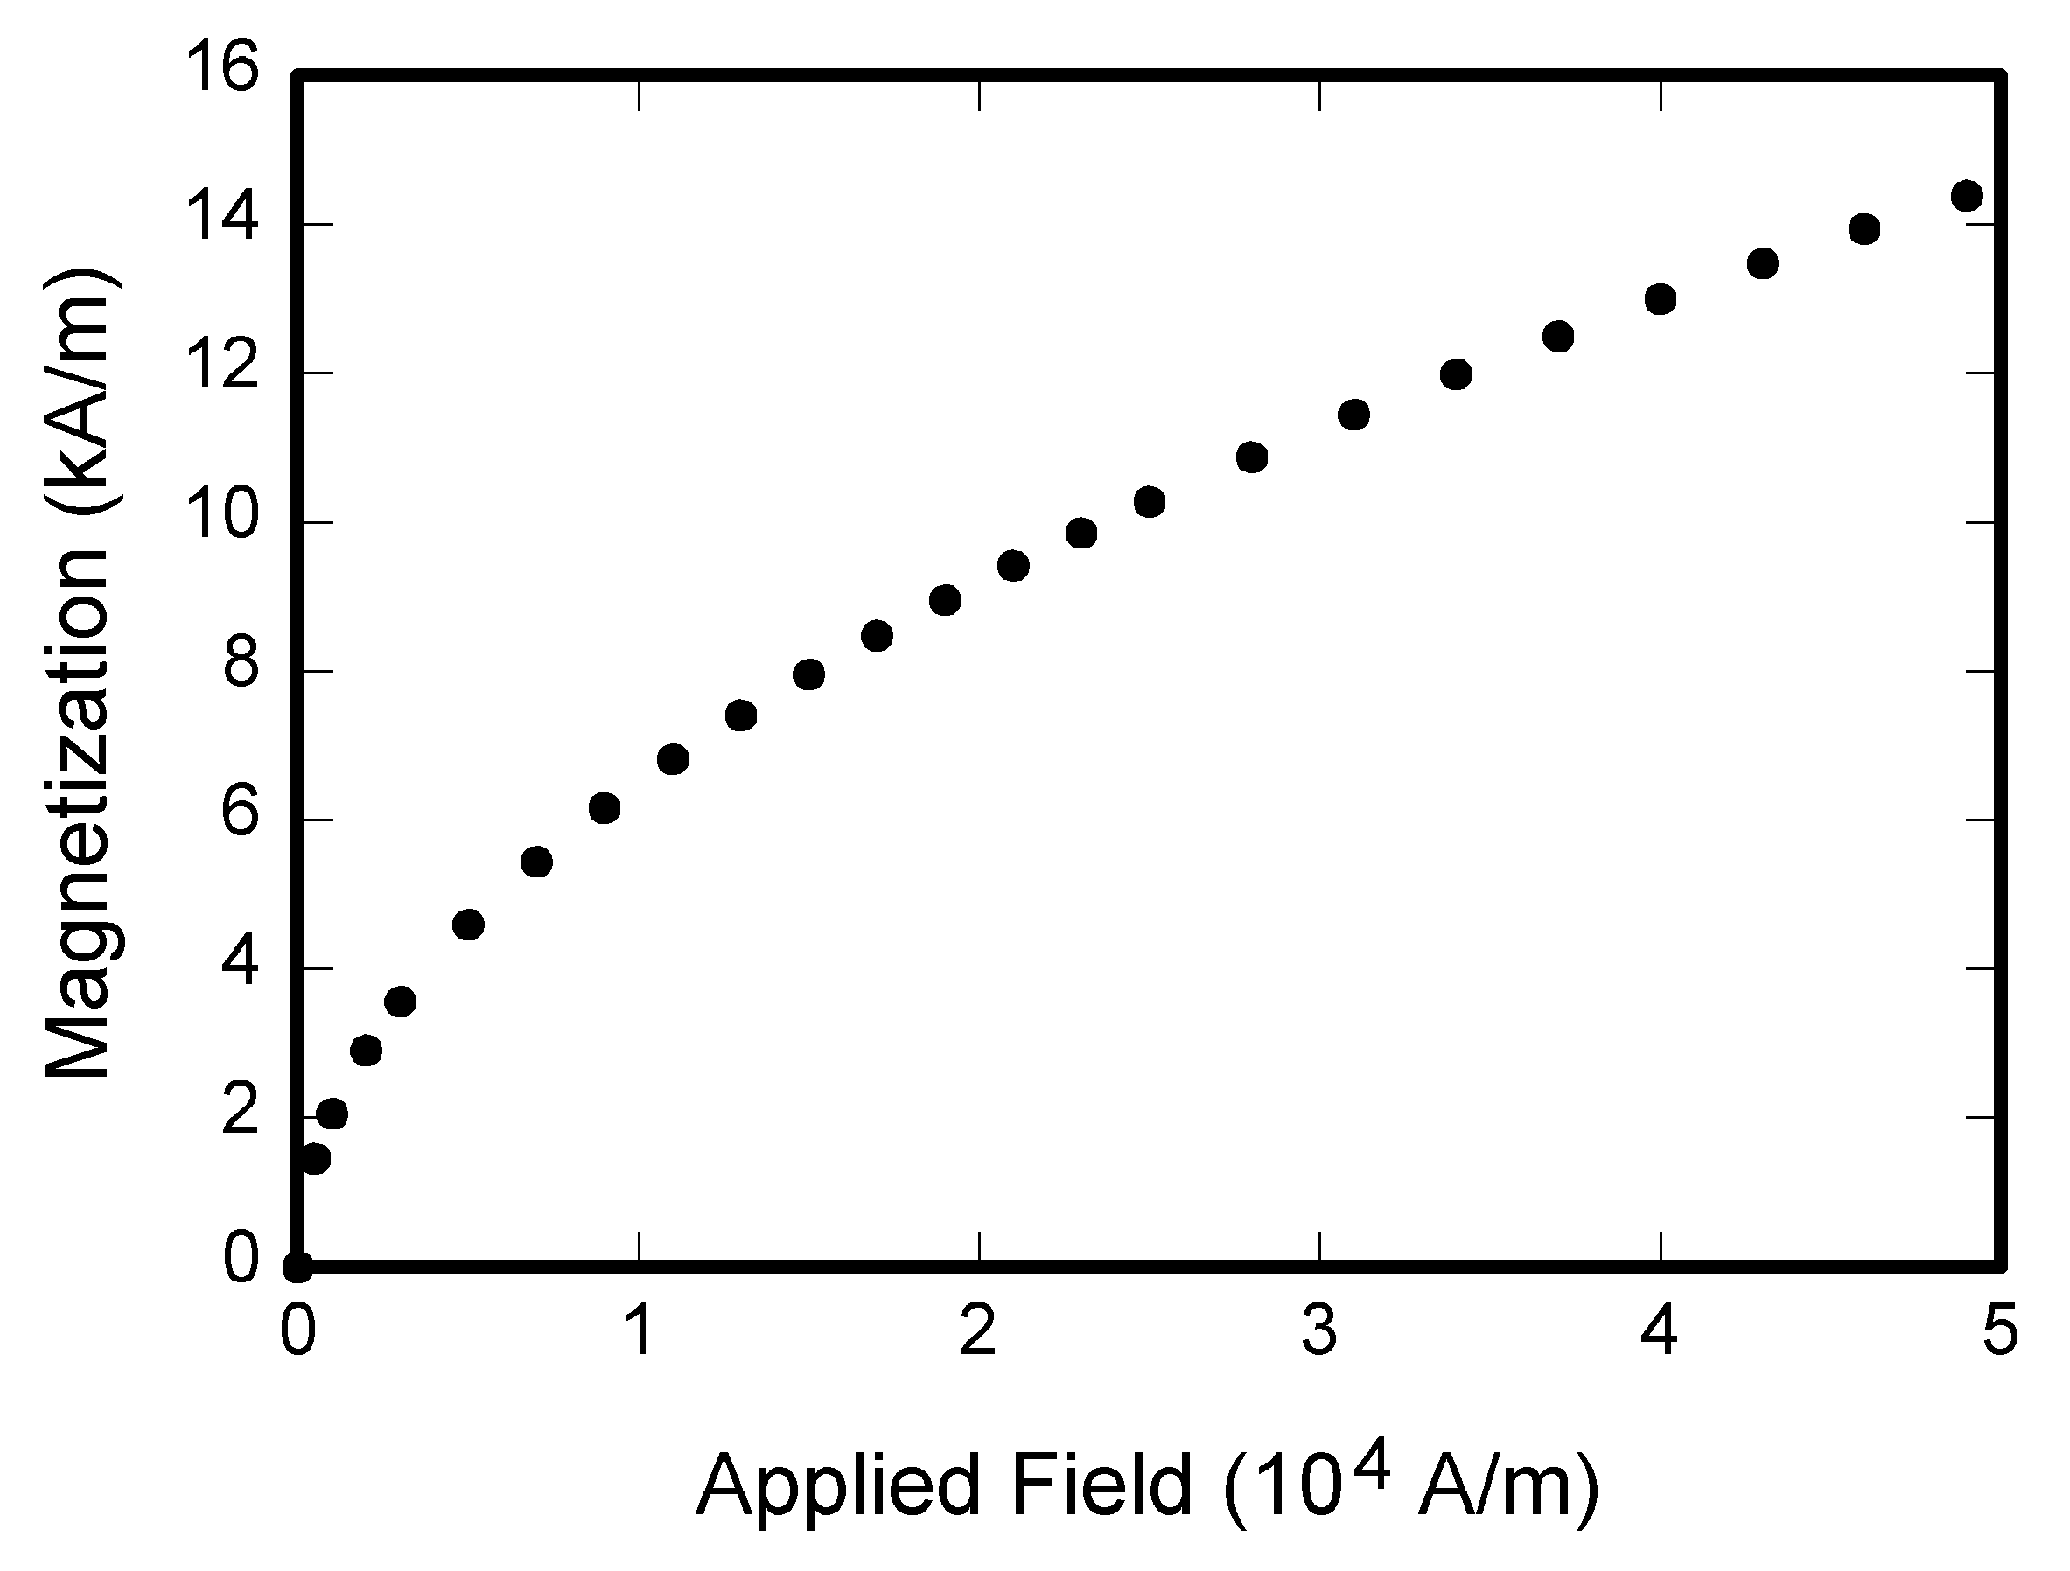
\includegraphics[width=\linewidth]{fig/fig1.png}
\caption{Adaptive Q-band scheduling. Preview risk increases band weights before aggressive steering, while residual monitoring delays weight release after the maneuver.}
\label{fig:qband_scheduler}
\end{figure}
% TODO（作者）：将 fig1.png 替换为自适应权重流程图。建议用少量模块画出 reference preview、band energy、feedback residual、asymmetric smoothing、scheduled weights 和 NMPC。

\subsection{Implementation Notes}
The Q-band module is model-agnostic. For a kinematic predictor, $a_{y,k}$ can be approximated from curvature or steering; for a dynamic predictor, it can be computed from $\dot v_y+v_xr$; for TruckSim or model-truck validation, it is evaluated from the predicted tracking response. In all cases, the controller suppresses the lateral excitation sequence rather than explicitly controlling the liquid state.

% TODO（作者）：后续补充最终控制频率、预测步长、求解器、平均/峰值求解时间、低速 PP 与高速 NMPC 的切换阈值。若篇幅紧张，可放入一行 implementation paragraph。


\section{Validation}

\subsection{5-Pins Simulation Setup}
The proposed controller was first evaluated in a 5-pins lane-change simulation. The reference path contains five consecutive double-lane-change maneuvers with the same lateral displacement of 3.5 m and progressively shorter maneuver durations, starting from 4 s. This setting produces a continuous risk gradient: the first two double lane changes are mild, the third is transitional, and the fourth and fifth contain strong lateral excitation. The controlled object follows the semi-trailer tank truck setting used in TruckSim validation, while the Q-band module only uses the predicted lateral-acceleration sequence in the controller.

Fifteen controller variants were compared, including baseline tracking, lateral-acceleration hard constraint, acceleration magnitude/difference penalties, fixed Q-band, preview-adaptive Q-band, feedback-assisted Q-band, and Q-band soft constraints. The main metrics are peak $|\LTR_{\mathrm{est}}|$, RMS LTR, peak lateral acceleration, RMS tracking error, and segment-wise tracking/safety indicators.

\begin{figure*}[!t]
\centering
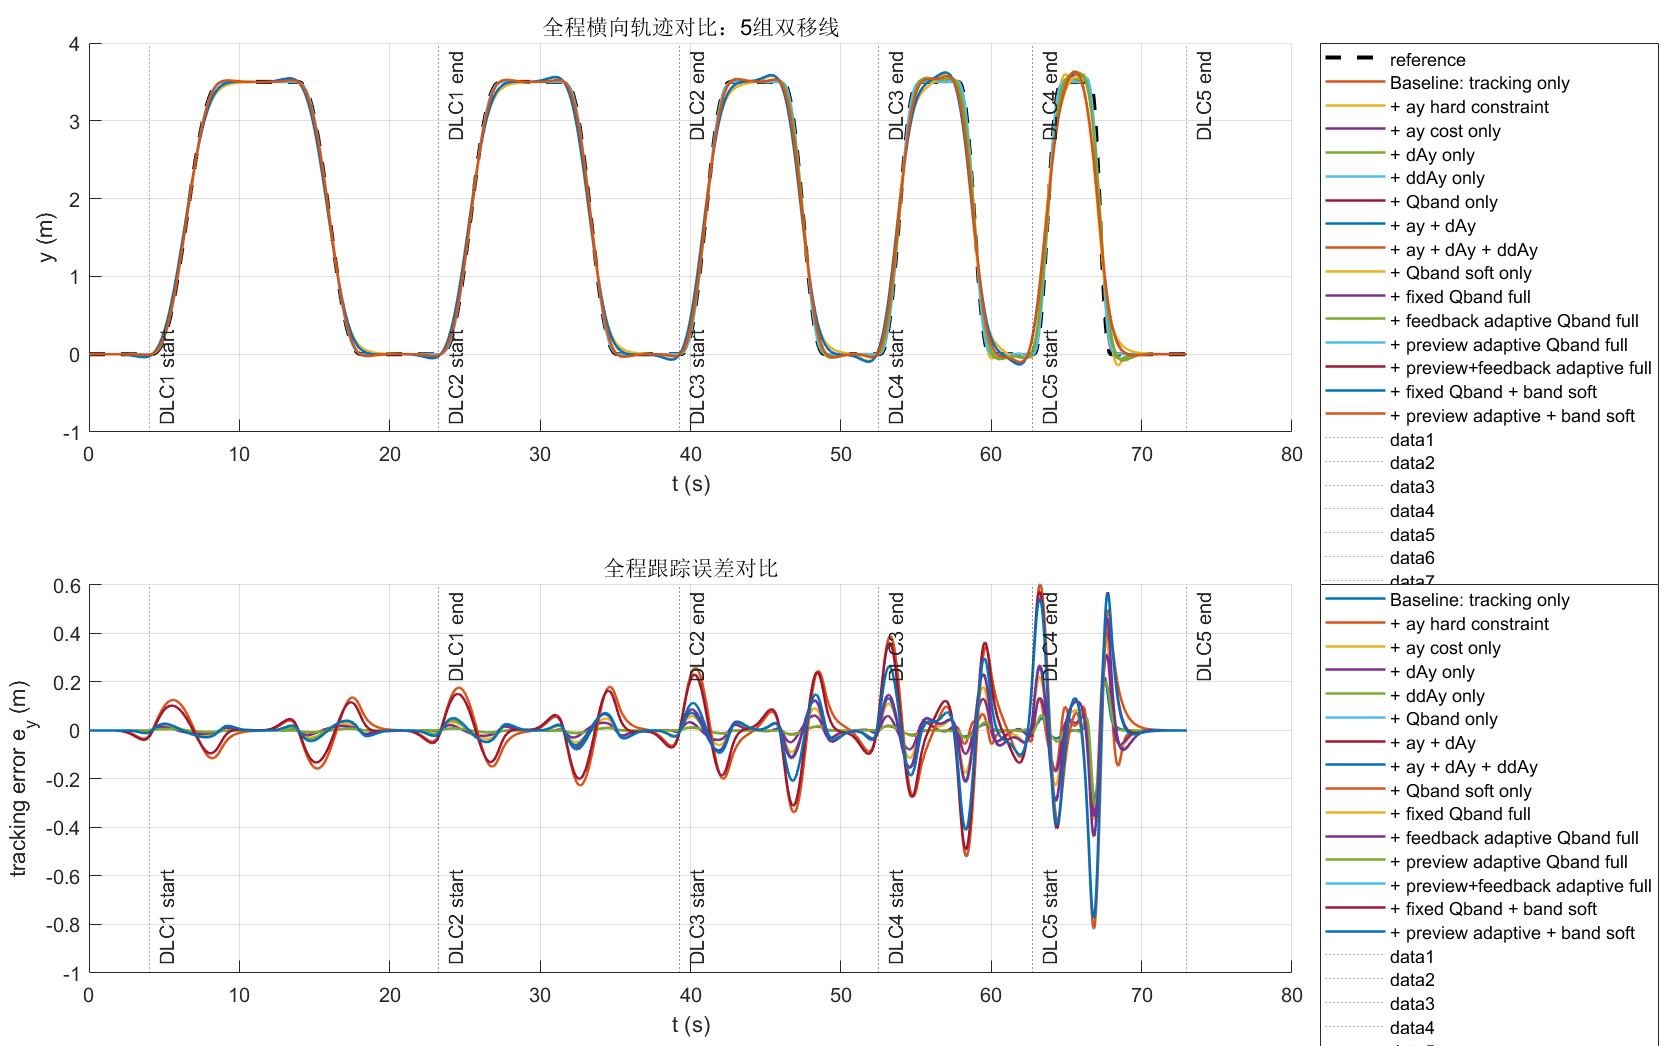
\includegraphics[width=0.98\textwidth]{fig/results1.png}
\caption{Five-pins tracking results. Low-risk segments are tracked closely by all methods; in the high-risk DLC4--DLC5 segments, Q-band and soft-constraint variants intentionally allow moderate path deviation to reduce rollover excitation.}
\label{fig:fivepins_tracking}
\end{figure*}
% TODO（作者）：当前 results1.png 是 MATLAB 粗图。建议最终版只保留 reference、baseline、fixed Q-band、preview Q-band、preview Q-band + soft 四条曲线；删除 data1/data2 等无效 legend；英文坐标轴和标题；用竖向浅色背景块标注 DLC1--DLC5，避免密集虚线和旋转文字。

\subsection{Simulation Results}
Fig.~\ref{fig:fivepins_tracking} shows that all controllers track the first three maneuvers with small errors. As the maneuver duration decreases, the baseline tracker maintains path accuracy but injects stronger oscillatory lateral acceleration. Q-band methods begin to relax tracking in DLC4 and DLC5, especially near the lane-return phases, where the predicted acceleration would otherwise fall into the critical band. The largest temporary tracking deviation is approximately xxx m in the current simulation and remains acceptable for the intended emergency maneuver envelope.

\begin{figure*}[!t]
\centering
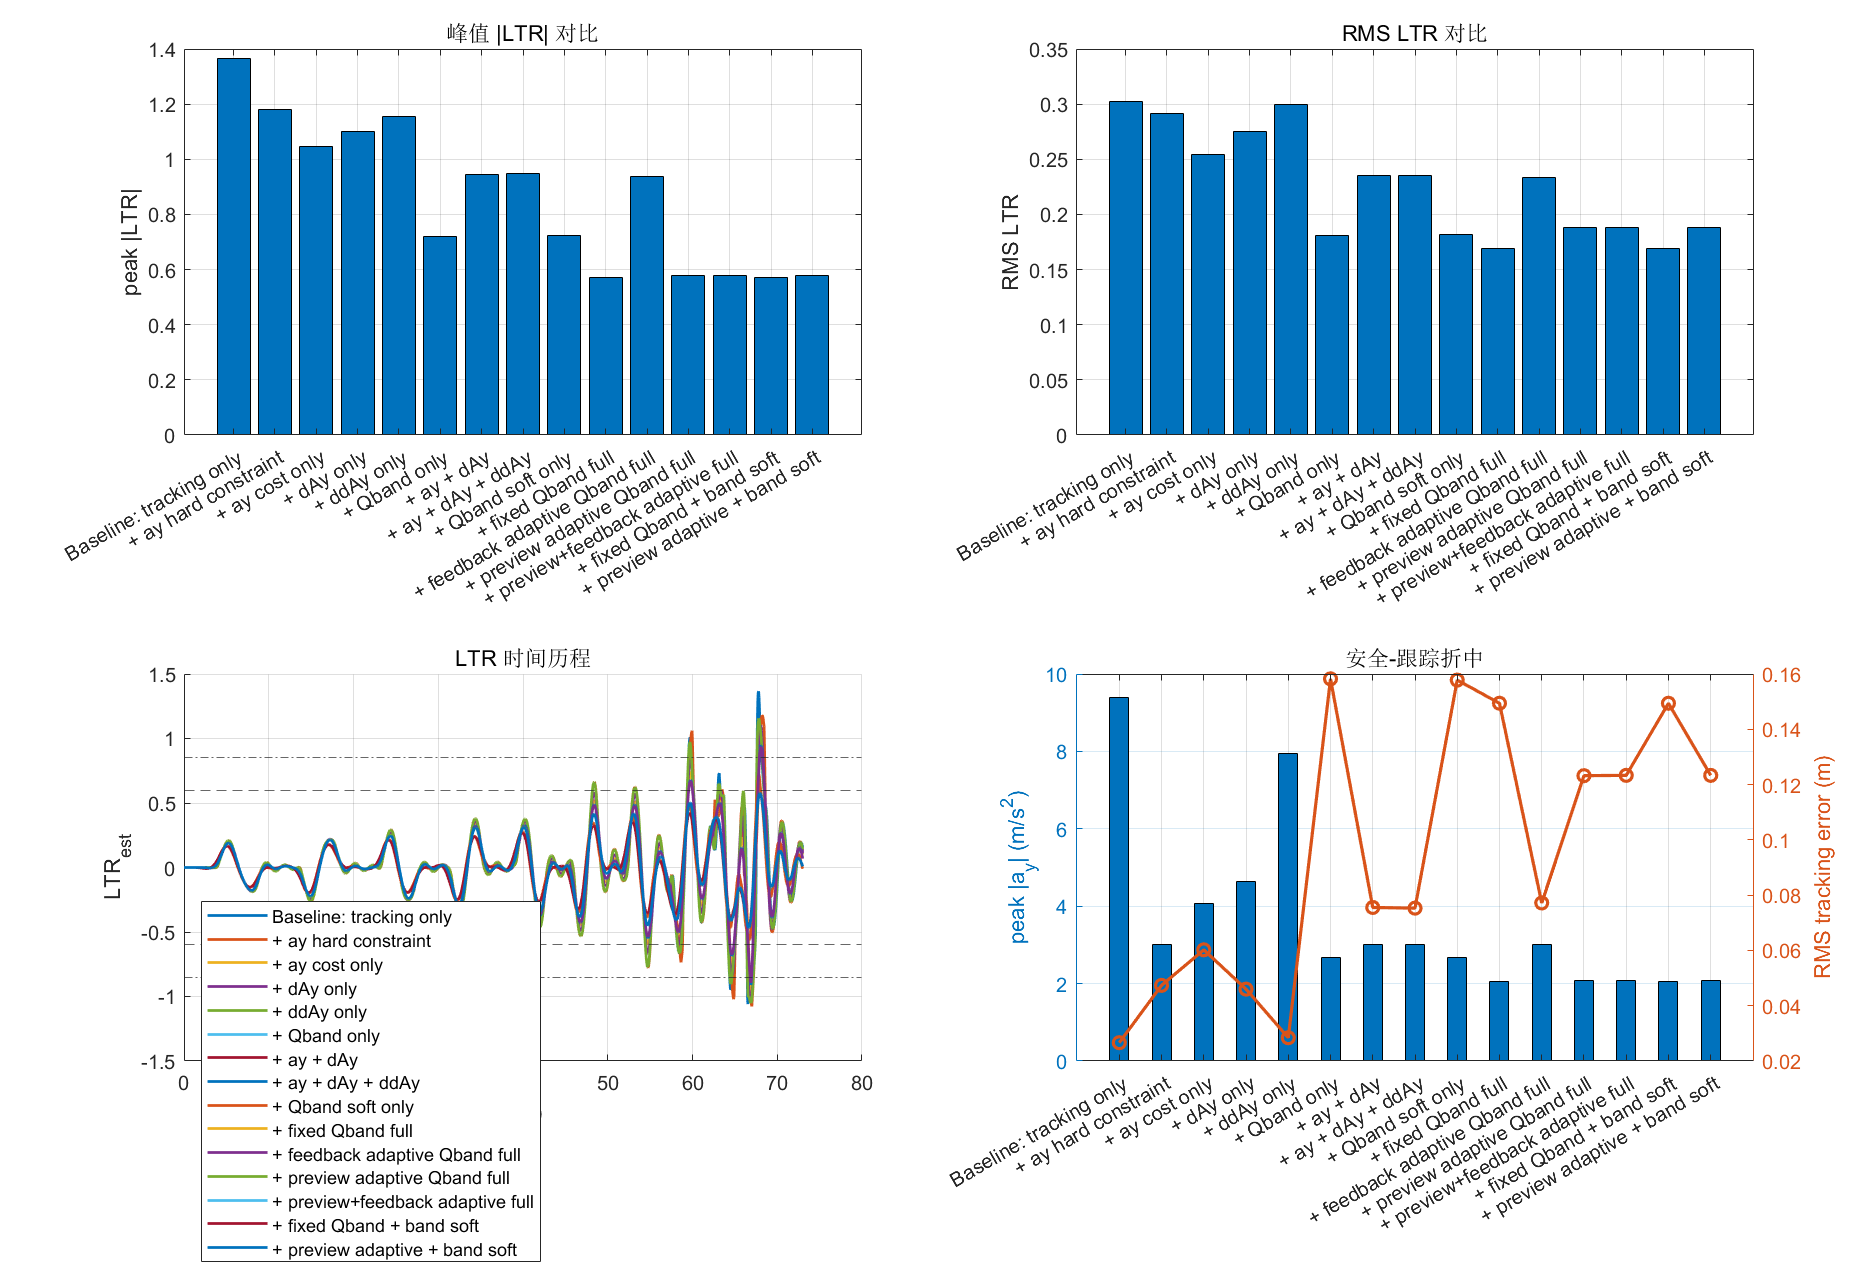
\includegraphics[width=0.98\textwidth]{fig/results2.png}
\caption{Ablation summary for the 5-pins simulation. Q-band-based variants reduce both peak $|\LTR_{\mathrm{est}}|$ and RMS LTR compared with baseline tracking, while the safety improvement is obtained at the cost of controlled tracking relaxation.}
\label{fig:fivepins_ablation}
\end{figure*}
% TODO（作者）：当前 results2.png 信息量太大。建议最终拆成两张或一个 2x2 组合图：peak |LTR|、RMS LTR、selected LTR time histories、safety-tracking Pareto。横轴 case 名称需要缩短，例如 Base、AyLim、Qband、Pre-Q、Pre-Q+Soft；安全阈值线建议统一标为 warning/danger。

The ablation results in Fig.~\ref{fig:fivepins_ablation} show three trends. First, the baseline peak $|\LTR_{\mathrm{est}}|$ reaches about xxx, exceeding the rollover-risk limit. Second, acceleration magnitude and difference penalties reduce part of the risk but cannot consistently suppress the critical high-risk segments. Third, fixed or adaptive Q-band variants reduce peak $|\LTR_{\mathrm{est}}|$ to approximately xxx--xxx and lower RMS LTR from xxx to xxx. The preview-adaptive and soft-constraint variants provide the most consistent reduction because the weights rise before DLC4--DLC5 and the optimizer is discouraged from placing energy in the critical band.

\begin{figure*}[!t]
\centering
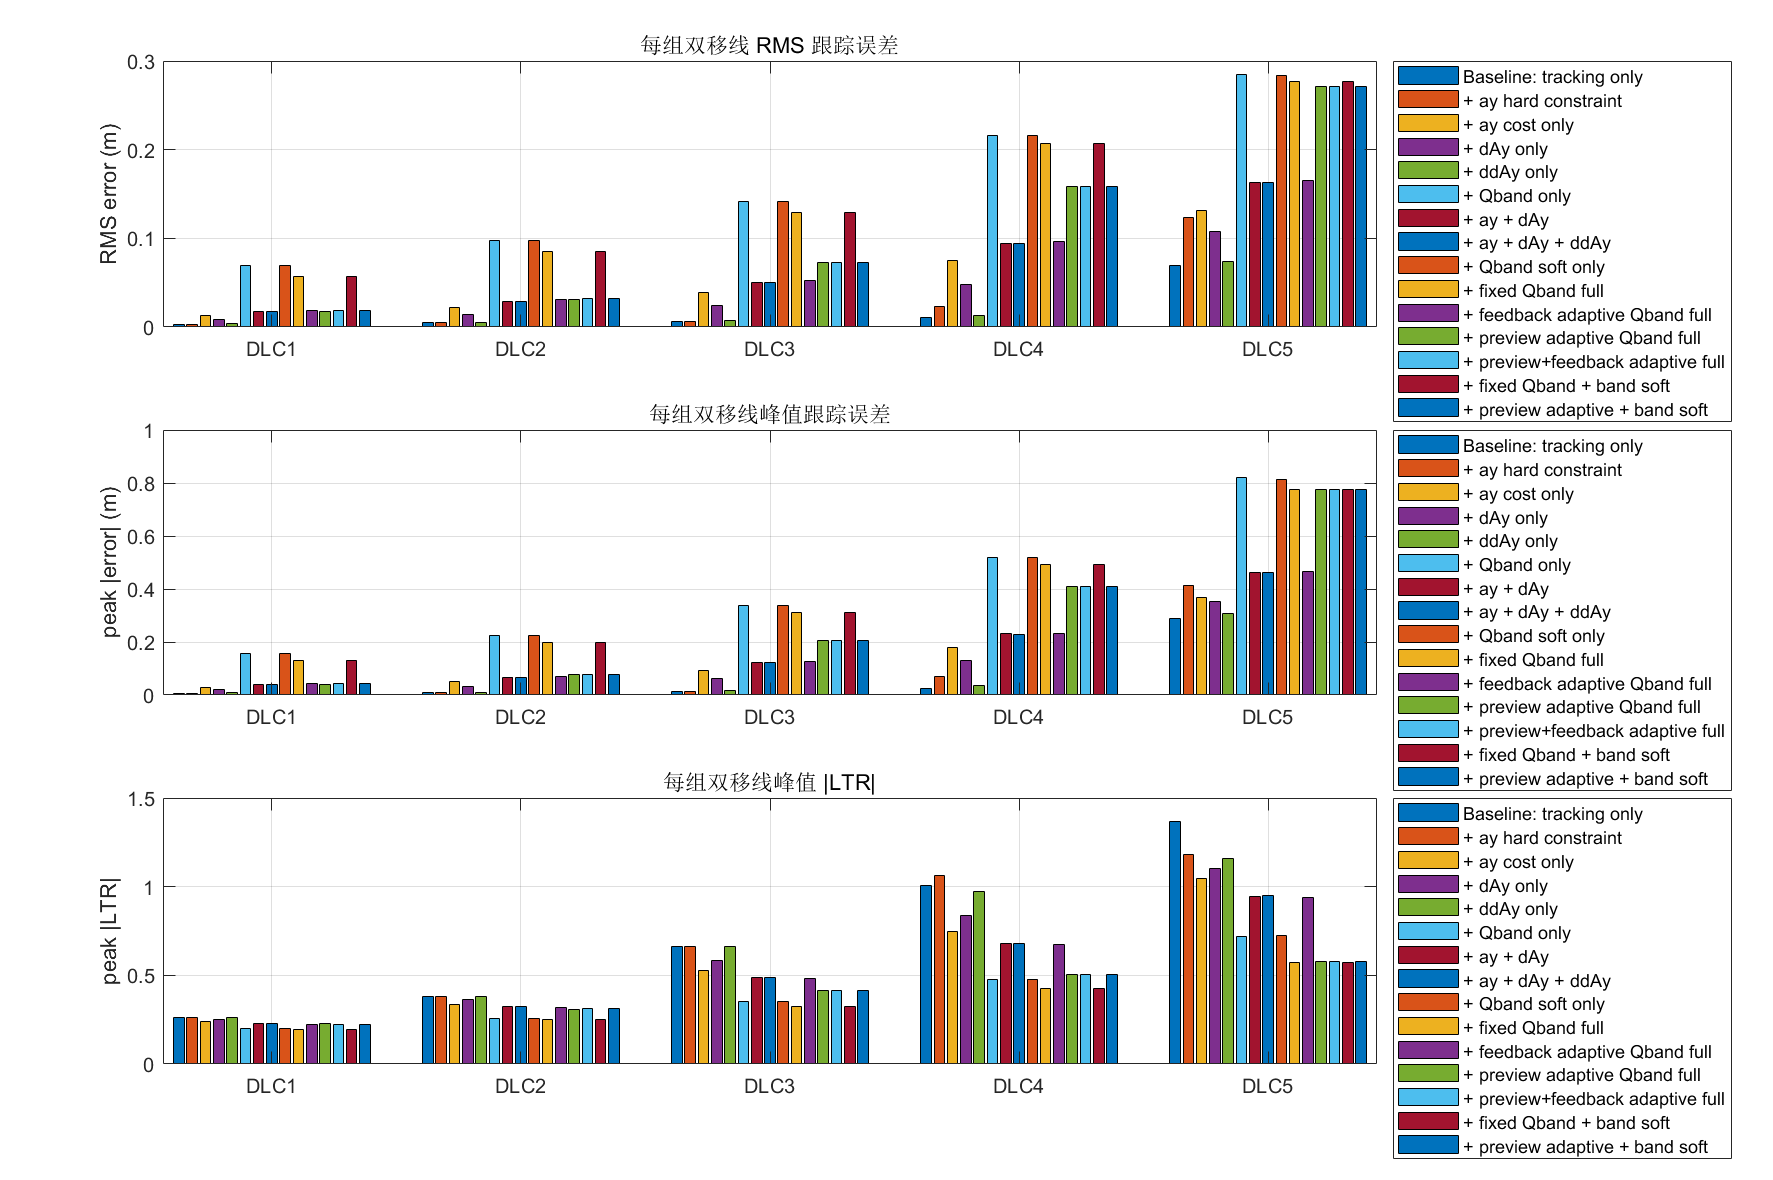
\includegraphics[width=0.98\textwidth]{fig/results3.png}
\caption{Segment-wise 5-pins metrics. The difference among methods is small in DLC1--DLC2, becomes visible in DLC3, and is dominated by the safety-tracking tradeoff in DLC4--DLC5.}
\label{fig:fivepins_segments}
\end{figure*}
% TODO（作者）：当前 results3.png legend 过大且重复三次。建议最终用分组柱状图只展示 4--5 个代表 case，并将 legend 放在图外上方一行；如果篇幅不够，可只保留第三行“每组双移线峰值 |LTR|”，把误差指标放入表格。

Segment-wise results in Fig.~\ref{fig:fivepins_segments} further confirm that Q-band ART is mainly activated in the dangerous sections. In DLC1 and DLC2, all methods have similar peak $|\LTR|$ and tracking error. In DLC3 the Q-band methods begin to separate from acceleration-only regularization. In DLC4 and DLC5, the baseline and acceleration-only strategies approach or exceed the risk threshold, while Q-band variants keep the peak risk proxy near xxx. This supports the design goal: low-risk segments remain close to ordinary tracking, and high-risk segments are reshaped to suppress dangerous lateral excitation.

\subsection{Model-Truck Experiment}
The 1:14 semi-trailer tank truck experiment was conducted to verify that the Q-band mechanism remains effective on a physical platform. The experiment used a double-lane-change or 5-pins-like reference path scaled according to the model-truck operating envelope. Baseline tracking and Q-band ART were compared under the same speed and filling-rate settings. The measured responses include path tracking, steering command, lateral acceleration, roll/yaw response, liquid-surface motion when available, and controller solve time.

The model-truck results show the same qualitative behavior as the simulation. Baseline tracking follows the reference more tightly but excites larger roll-slosh motion, and the anti-roll support/contact or rollover-risk proxy reaches xxx. Q-band ART reduces the peak risk proxy by xxx\%, keeps the liquid/roll response within xxx, and increases RMS tracking error from xxx m to xxx m. The controller average and peak solve times are xxx ms and xxx ms, respectively, satisfying the real-time requirement of the experimental platform.

% TODO（作者）：这里后续需要插入模型车实验总图。建议包含：平台照片、实验路径、baseline vs Q-band 轨迹、风险代理/LTR、液面或侧倾响应、求解时间。若没有液面可靠识别，就明确写“liquid-surface motion is used only for qualitative video confirmation”。

\begin{table}[!t]
\caption{Validation Summary With Replaceable Results}
\label{tab:validation_summary}
\centering
\begin{tabularx}{\linewidth}{lXXX}
\toprule
Case & Peak risk proxy & RMS error & Solve time\\
\midrule
Simulation baseline & xxx & xxx m & xxx ms\\
Simulation Q-band ART & xxx & xxx m & xxx ms\\
Model-truck baseline & xxx & xxx m & --\\
Model-truck Q-band ART & xxx & xxx m & xxx ms\\
\bottomrule
\end{tabularx}
\end{table}
% TODO（作者）：表中 peak risk proxy 最终统一成 peak |LTR_est|、peak roll rate 或 support-contact indicator 之一；仿真和模型车如果指标不同，需要在表注里说明，避免直接比较不同定义的数值。


\section{Conclusion}
This paper proposed Q-band ART, an adaptive frequency-band suppression method for anti-rollover tracking of semi-trailer tank trucks. Instead of using liquid sloshing states or wheel-load-based LTR as online controller states, it suppresses predicted lateral-acceleration energy in critical vehicle-liquid bands. A reduced roll-sloshing model provides the frequency-domain safety interpretation, and the Q-band term is integrated with acceleration smoothing, soft constraints, preview-adaptive scheduling, ESO compensation, and hitch-angle-based parameter scheduling.

Continuous five-pins co-simulation and independent-DLC ablation show that Q-band ART avoids rollover where pure preview tracking and acceleration-amplitude limiting fail. Compared with full-state active steering, it provides comparable anti-rollover tracking with lower dependence on liquid-state observation, trailer-side feedback, and high-dimensional online models. The results indicate that input-side critical-band suppression is a practical complement to explicit rollover-state constraints. Future work will refine critical-band calibration across filling rates and integrate Q-band scheduling with combined steering and braking control.


\bibliographystyle{IEEEtran}
\bibliography{main}


\vspace{12pt}
% \color{red}
% IEEE conference templates contain guidance text for composing and formatting conference papers. Please ensure that all template text is removed from your conference paper prior to submission to the conference. Failure to remove the template text from your paper may result in your paper not being published.

\end{document}
